\documentclass[11pt, aspectratio=169]{beamer}

% Common imports and commands

\usepackage[utf8]{inputenc}
\usetheme{Madrid}
%\usecolortheme{beaver}
 
% Fix to beamer don't having `figure*'
% See [here](https://tex.stackexchange.com/questions/16527/redefining-figure-for-beamer)
\newenvironment{figure*}%
{\begin{figure}}
{\end{figure}}
\usepackage{common}
\usepackage{biblatex} 
\DeclareFontShape{OT1}{cmss}{b}{n}{<->ssub * cmss/bx/n}{} 
\bibliography{main.bib}

%Information to be included in the title page:
\title{\textbf{Reinforcement Learning-based Hierarchical Seed Scheduling for Greybox Fuzzing}}
\author[Rong]{\textbf{Yuyang(Peter) Rong}}
\institute[UC Davis]{
  University of California, Davis \\ PtrRong@ucdavis.edu
}

\date[Sept 2021]
{Sept 2021}

\begin{document}


% \frame{\titlepage}

\begin{frame}
	\frametitle{Introduction: Greybox fuzzing}
	% What is greybox fuzzing, what is the workflow, what is the decision choices
	\begin{figure}
    \centering
    \begin{tikzpicture}[
            auto,
            box/.style = {
                    draw,rounded corners,blur shadow,fill=white,
                    align=center,text width=3cm,
                    node distance=5mm
                },
        ]
        \node [box] [minimum width=5cm, text width=5cm](source) {Source code(C, C++, ...)};
        \node [draw = none, below = 6cm of source] {\textbf{Greybox fuzzer}};
        \draw[thick,dotted] ($(source.south west)+(-0.5,-0.4)$)  rectangle ($(source.south west)+(+14.5,-6.5)$);

        \pause
        \node [box] [below = of source](IR) {Intermediate representation (IR)};
        \node [box, right= 1cm of IR] (instrumentation) {Instrumentation};
        \node [box, below=of instrumentation] (P) {Testing program};
        \path (source) edge[cfgedge] node[left]{Compiler frontend}  (IR);
        \path (IR) edge[cfgedge] (instrumentation);
        \path (instrumentation) edge[cfgedge] node[right] {Compiler backend} (P);
        \pause
        \node [box, below = 3cm of P] (S) {Seed store};
        \node [box, right = 1cm of S] (I) {Initial seed};
        \path (I.west) edge[cfgedge] (S.east);
        \pause
        \node [box, below left = 1cm and 2cm of P] (M) {Mutation};
        \node [box, below right = 1cm and 2cm of P] (B) {Behavior observation};
        \node [above=of B] (D) {};
        \path (P.south east) edge[cfgedge, bend left] (B.north west);
        \path (B.south west) edge[cfgedge, bend left, align = left] node[above] {Has new \\ behavior} (S.north east);
        \path (S.north west) edge[cfgedge, bend left, align = left] node[above] {Seed \\ selection} (M.south east);
        \path (M.north east) edge[cfgedge, bend left, align = left] node[below] {New \\ input} (P.south west);
        \path (B.north) edge[cfgedge, bend left, align=left] node[right] {Discard if no \\ new behavior} (D.south);
        \pause
    \end{tikzpicture}
\end{figure}
	\begin{textblock}{8}(9, 2)
		\begin{itemize}
			\item \textbf{How is ``new behavior'' defined?}
			\item \textbf{How do we ``mutate'' input?}
		\end{itemize}
	\end{textblock}
\end{frame}
\begin{frame}
	\frametitle{Background: American Fuzzy Lop (AFL) \footfullcite{AFL}}
	% How do state of the art AFL solve this?
	\begin{itemize}
		\item``Mutation'' is purely random.
		\item Many ways to define ``New behavior'', AFL uses branch count.
	\end{itemize}
	\pause
	\begin{figure}[t]
  \centering
  \begin{subfigure}[b]{0.24\textwidth}
    \begin{tikzpicture}[auto]
      \tikzstyle{every node} = [align=center, node distance=1.3cm]
      \node [draw, circle, minimum size=0.75cm] (A)  {$A$};
      \node [above of=A, node distance=1cm] (in)  {};
      \node [draw, circle, minimum size=0.75cm, below left of = A, node distance=1.7cm] (B1) {$B_1$};
      \node [draw, circle, minimum size=0.75cm, below right of=A, node distance=1.7cm] (B2) {$B_2$};
      \node [draw, circle, minimum size=0.75cm, below left of = B2, node distance=1.7cm] (C) {$C$};
      \node [below of=C, node distance=1cm] (out) {};

      \path (in) edge[cfgedge,] node {\footnotesize in} (A);
      \path (A) edge[cfgedge, bend right] node[above left] {\texttt{a}} (B1);
      \path (B1) edge[cfgedge, bend right] node [left]{\texttt{c}} (A);
      \path (B2) edge[cfgedge, bend left] node[right] {\texttt{e}} (C);
      \path (B1) edge[cfgedge, bend right] node[right] {\texttt{d}} (C);
      \path (A) edge[cfgedge, bend left] node[above right] {\texttt{b}} (B2);
      \path (C) edge[cfgedge,] node {\footnotesize out} (out);
    \end{tikzpicture}
    \caption{Get Control Flow Graph (CFG) from IR.}
  \end{subfigure}
  \pause
  \begin{subfigure}[b]{0.4\textwidth}
    \begin{tikzpicture}[auto, draw]
      \node (B) [rectangle, align=left]{
        $ID(A) = \texttt{0x0001234}$ \\
        $ID(B_1)=\texttt{0x000beaf}$ \\
        $ID(B_2)=\texttt{0x0005678}$ \\
        $ID(C) = \texttt{0x0009c89}$ \\
      };
      \node (E) [below of = B, rectangle, align=left, node distance = 2cm] {
        $ID(\texttt{a}) = (ID(B_1) >> 1) \text{ xor }ID(A)$\\
        $ID(\texttt{c}) = (ID(A) >> 1) \text{ xor }ID(B_1)$\\
        $\cdots$
      };
      \path(B) edge[cfgedge] (E);
    \end{tikzpicture}
    \caption{Randomly assign block ID (Instrumentation) and compute edge ID (Runtime).}
  \end{subfigure}
  \pause
  \begin{subfigure}[b]{0.24\textwidth}
    \begin{tikzpicture}[
        auto,
        mem/.style = {rectangle, draw=black!50, minimum width=16mm,
                minimum height = 4mm},
    ]
    \node (c) [rectangle, align=left]{$ID(\texttt{c}) = \texttt{\textbf{b7b5}}$};

    \node  [mem, draw, below = 5mm of c] (0) {};
    \node  [left = 1mm of 0] (00) {$\texttt{0x0000}$};
    \node  [mem, draw, below = 0mm of 0] (1) {};
    \node  [left = 1mm of 1] (10) {$\texttt{0x0001}$};
    \node  [mem, draw, below = 0mm of 1] (m) {$\cdots$};
    \node  [left = 1mm of m] (m0) {$\cdots$};
    \node  [mem, draw, below = 0mm of m] (b7b5) {};
    \node  [left = 1mm of b7b5] (b7b50) {$\texttt{\textbf{0xb7b5}}$};
    \node  [mem, draw, below = 0mm of b7b5] (mm) {$\cdots$};
    \node  [left = 1mm of mm] (mm0) {$\cdots$};
    \node  [mem, draw, below = 0mm of mm] (fe) {};
    \node  [left = 1mm of fe] (fe0) {$\texttt{0xfffe}$};
    \node  [mem, draw, below = 0mm of fe] (ff) {};
    \node  [left = 1mm of ff] (ff0) {$\texttt{0xffff}$};

    \path (c) edge[cfgedge, bend left] (b7b50);
\end{tikzpicture}
    \caption{Using edge ID to index a 64KB branch count table.}
  \end{subfigure}
\end{figure}
\end{frame}
\begin{frame}
	\frametitle{Background: American Fuzzy Lop (AFL)}
	\begin{minipage}[t]{0.49\linewidth}
		\begin{itemize}
			\item Each byte in the table represents 8 possible ranges of hit count.
			      \begin{itemize}
				      \item $\texttt{0x00} \rightarrow 0..0 $
				      \item $\texttt{0x01} \rightarrow 1..1 $
				      \item $\cdots$
				      \item $\texttt{0x08} \rightarrow 4..7 $
				      \item $\texttt{0x10} \rightarrow 8..15 $
				      \item $\cdots$
				      \item $\texttt{0x80} \rightarrow 128+$
			      \end{itemize}
			\item Every run local branch counting table is compared (bitwise xor) then merged (bitwise or) with global table.
		\end{itemize}
	\end{minipage}
	\hfill
	\begin{minipage}[t]{0.49\linewidth}
		\begin{figure}[t]
			\centering
			\begin{tikzpicture}[
        auto,
        mem/.style = {rectangle, draw=black!50, minimum width=16mm,
                minimum height = 4mm},
    ]
    \node (c) [rectangle, align=left]{$ID(\texttt{c}) = \texttt{\textbf{b7b5}}$};

    \node  [mem, draw, below = 5mm of c] (0) {};
    \node  [left = 1mm of 0] (00) {$\texttt{0x0000}$};
    \node  [mem, draw, below = 0mm of 0] (1) {};
    \node  [left = 1mm of 1] (10) {$\texttt{0x0001}$};
    \node  [mem, draw, below = 0mm of 1] (m) {$\cdots$};
    \node  [left = 1mm of m] (m0) {$\cdots$};
    \node  [mem, draw, below = 0mm of m] (b7b5) {};
    \node  [left = 1mm of b7b5] (b7b50) {$\texttt{\textbf{0xb7b5}}$};
    \node  [mem, draw, below = 0mm of b7b5] (mm) {$\cdots$};
    \node  [left = 1mm of mm] (mm0) {$\cdots$};
    \node  [mem, draw, below = 0mm of mm] (fe) {};
    \node  [left = 1mm of fe] (fe0) {$\texttt{0xfffe}$};
    \node  [mem, draw, below = 0mm of fe] (ff) {};
    \node  [left = 1mm of ff] (ff0) {$\texttt{0xffff}$};

    \path (c) edge[cfgedge, bend left] (b7b50);
\end{tikzpicture}
		\end{figure}
	\end{minipage}
\end{frame}

\begin{frame}
	\frametitle{Background: Be more sensitive \footfullcite{241986}}
	\begin{itemize}
		\item You can be less sensitive by using block coverage.
		\item Add calling context or N-gram edge coverage to be more sensitive.
		\item The more sensitive, the better?
	\end{itemize}
	\begin{figure}
		\centering
		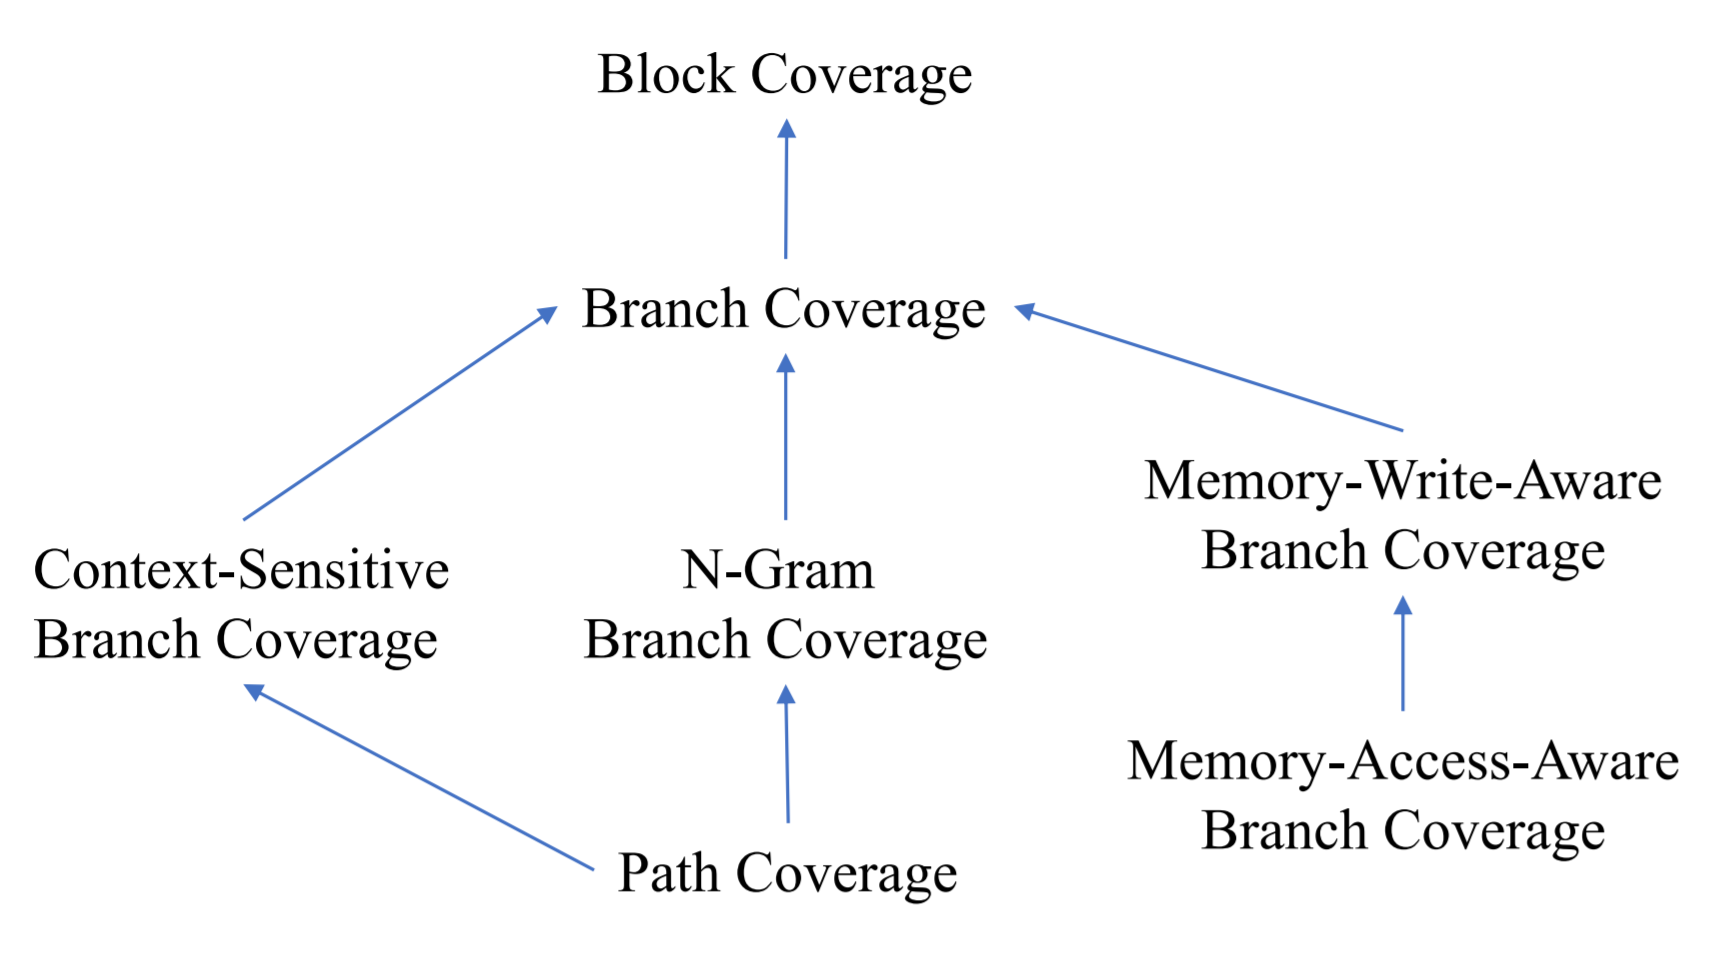
\includegraphics[width=0.5\textwidth]{figs/lattice.png}
	\end{figure}
\end{frame}

\begin{frame}[fragile]
	\frametitle{Background: Seed explosion}
	\begin{minipage}[t]{0.49\linewidth}
		\begin{lstlisting}[
				language = C, 
				xleftmargin=1cm,
				basicstyle=\footnotesize\ttfamily
			  ]
int n = getc();
int sum = 0;
for (int i=0; i<n; i++) {
	sum += getc();
}
			  \end{lstlisting}
		\begin{itemize}
			\item Seed 1: 0x01, 0x01
			\item Seed 2: 0x02, 0x01, 0x02
			\item Seed 3: 0x03, 0x01, 0x02, 0x03
		\end{itemize}
	\end{minipage}
	\begin{minipage}[t]{0.49\linewidth}
		\begin{itemize}
			\item Function coverage: It's the same function so 3 seeds are the same.
			\item Block coverage: Same blocks get executed so 3 seeds are the same.
			\item Edge coverage: Seed 1 and 2 are different (loop back edge executed in seed 2), 2 and 3 are the same.
			\item $\infty$ gram: Seeds are different as long as n is different.
		\end{itemize}
	\end{minipage}
\end{frame}
\begin{frame}
	\frametitle{Design: high level idea}
	\begin{itemize}
		\item Seed store is a FIFO queue in most AFL based fuzzers, seed explosion could greatly impact fuzzing performance.
		\item A seed has two objectives:
		      \begin{itemize}
			      \item Explore the code, ``exercising an entirely different function'', need less sensitive feedback.
			      \item Exploit the code, focus on solving a particular branch predicate, need more sensitive feedback.
		      \end{itemize}
		\item This is similar to Multi-armed bandit (MAB) problem\footfullcite{10.1145/2508859.2516736}.
	\end{itemize}
\end{frame}

\begin{frame}
	\frametitle{Design: multi level coverage metrics(Sec III)}
	\begin{itemize}
		\item $M_F$: Seeds with the same function coverage
		\item $M_E$: Seeds with the same edge coverage
		\item $M_D$: Seeds with the same hamming distance
	\end{itemize}

	\begin{figure}
		\centering
		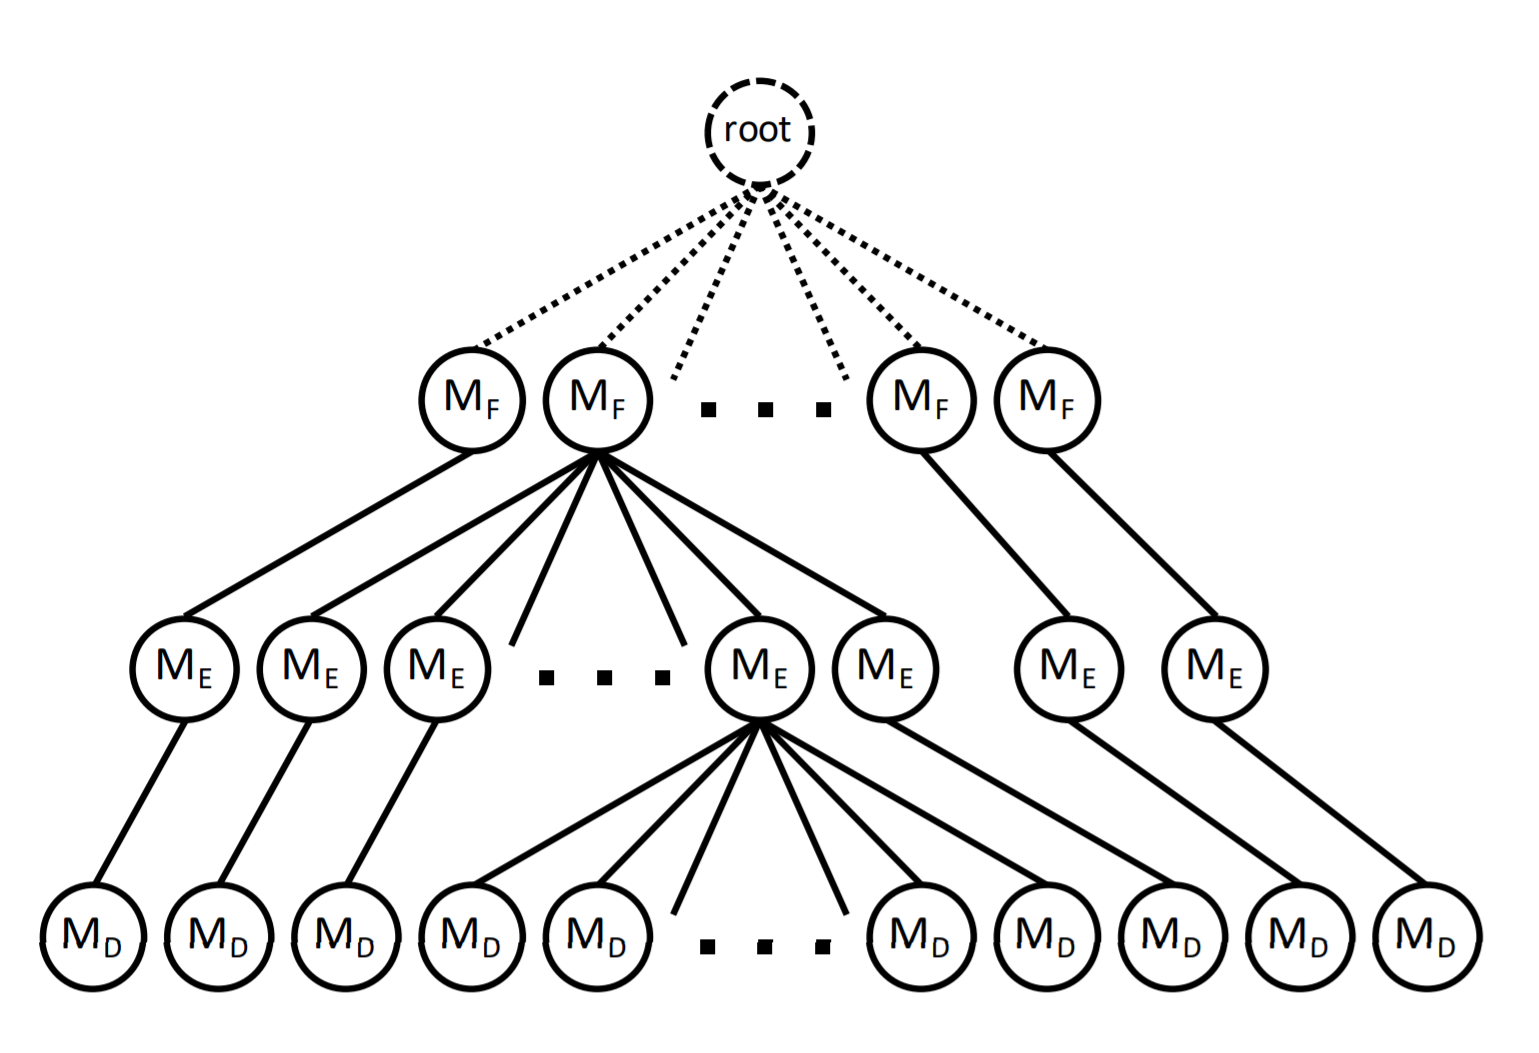
\includegraphics[width=0.5\textwidth]{figs/seedtree.png}
	\end{figure}

	Without FIFO queue, how do we know which seed to take next?
\end{frame}

\begin{frame}
	\frametitle{Design: Hierarchical seed scheduling}
	\begin{itemize}
		\item Seed are scheduled based on their score (Algorithm 3)
		\item $\texttt{Score}(a) = \texttt{Rareness}(a) \times (\texttt{Reward}(a) + \texttt{Uncertainty}(a))$
		\item $\texttt{Rareness}(a)$: Measures how rare is the seed? (Equation 6, 7)
		\item $\texttt{Reward}(a)$: How much reward has the seed gained? (Equation 4)
		\item $\texttt{Uncertainty}(a)$: Radius of the upper confidence interval of \texttt{Reward} (Equation 5)
	\end{itemize}
\end{frame}
\begin{frame}
    \frametitle{Evaluation}
\end{frame}
\begin{frame}
    \frametitle{Reinforcement Learning\footfullcite{sutton2018reinforcement}}
    \begin{figure}
        \centering
        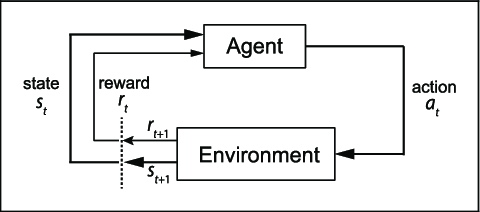
\includegraphics[height=0.3\textheight]{figs/rl.png}
    \end{figure}
\end{frame}

\begin{frame}
    \frametitle{Multi armed bandit (Chp 2)}
    \begin{itemize}
        \item Stateless, tradeoff between exploration and exploitation.
        \item Action value function $Q_t(a)$: at time $t$, action $a$'s expected reward.
        \item Solutions:
              \begin{itemize}
                  \item $\epsilon$-greedy: give $\epsilon$ chance of random selection(exploration), otherwise greedily chose best arm(exploitation) (Chp 2.3)
                  \item Upper-Confidence-Bound (Used in last paper we discussed\footfullcite{wangreinforcement}) (Chp 2.7)
              \end{itemize}
    \end{itemize}
\end{frame}

\begin{frame}
    \frametitle{Markov Desicion Process (Chp 3)}
    \begin{itemize}
        \item ``The reward signal is your way of communicating to the robot \textit{what} you want it to achieve, not \textit{how} you want it achieved.''
        \item ``In general, actions can be any decisions we want to learn how to make, and the states can be anything we can know that might be useful in making them.''
        \item Policy: a distribution of actions to take. $\pi(a|s)$: Given current state $s$, the probablity of selecting action $a$.
        \item State function: $v_\pi(s)$: given policy $\pi$, how good are we to be at state $s$?
        \item We want to find the best \textbf{espected return}, so it's not really greedy.
        \item Discount history reward for math and engineering reasons:
              \begin{itemize}
                  \item Avoid infinite amount when $t\rightarrow\infty$.
                  \item History may not reflect the future, e.g., a fuzzed seed may not generate the same reward it used to.
              \end{itemize}
    \end{itemize}
\end{frame}

\begin{frame}
    \frametitle{Suppose we have a perfect model... Dynamic Programming (Chp 4)}
    \begin{itemize}
        \item We have a perfect model, i.e. we don't need to interact with the environment to know the reward, $v_\pi(s)$ can be computed in Formula 4.4.
        \item Start with a random policy, iteratively update value function, then derive a new policy (Example 4.1).
        \item Generalized Policy Iteration(GPI) (Sec 4.4)
    \end{itemize}
\end{frame}

\begin{frame}
    \frametitle{We don't really have a model... Monte Carlo Methods (Chp 5)}
    \begin{itemize}
        \item Problem is too complicated(fuzzing), or simple problem with hard model(Blackjack)
        \item $v_\pi(s)$ is not good enough, since most states can't be fully experimented, therefore we work on $q_\pi(s, a)$.
        \item Each game is an episode, finish an episode and reversely update $q_\pi(s, a)$.
              \begin{itemize}
                  \item On-policy: Explore the episode with our derived policy, but how do we explore? Exploring start(Chp 5.3) or $\epsilon$-greedy (Chp 5.4).
                  \item Off-policy: Explore the episode using another policy, but how to reflect the reward on our policy? Importance Sampling (Chp 5.5)
              \end{itemize}
    \end{itemize}
\end{frame}

\begin{frame}
    \frametitle{We don't want to finish a game too... Temperal Difference (Chp 5, 6)}
    \begin{itemize}
        \item Can be implemented online (compared to Monte Carlo), doesn't need a model (compared to DP)
        \item Immediately update $v_\pi(s)$ after a step. (Formula 6.2):
              \begin{itemize}
                  \item On-policy SARSA: Update based on the \textbf{next} state-action pair. (Formula 6.7)
                  \item Off-policy Q-learning: Update based on the \textbf{best} state-action pair. (Formula 6.8)
              \end{itemize}
        \item Chp 7: n-step bootstrapping. Tradeoff between TD and monte Carlo, update based on next n steps.
    \end{itemize}
\end{frame}

\begin{frame}
    \frametitle{Tabular method and approximate solution}
    \begin{itemize}
        \item Tabular: You can write state-action pair in a table and update each entry based on your experience.
        \item If the table is too large, i.e. too many states, you have to approximate a state value using known info.
        \item Gradient policy method directly approximates the policy.
    \end{itemize}
\end{frame}

\begin{frame}
    \frametitle{Gradient policy method\footfullcite{sutton1999policy}}
    \begin{itemize}
        \item Policy is parameterizxed by $\mathbf{\theta}$, i.e. $\pi(a|s,\mathbf{\theta})$.
        \item $\mathbf{\theta}$ can be a lot of things. For example, it can ba all weights of a deep artifical neural network.
        \item Performance measure $J(\mathbf{\theta}) = v_{\pi_\mathbf{\theta}}(s_0)$, i.e. how good is the initial state?
        \item Policy gradient theorem makes $\nabla J$ computable (Chp 13.2)
    \end{itemize}
\end{frame}
\end{document}
